\section{Basics of computer science, part \rom{1}}
\subsection*{Data and Digital Storage}
The logic and mathematics of the digital world are essential tools in computer science. Since in the most basic way computers work with binary digits (0s and 1s), a basic grasp of data representation and arithmetics in binary base in extremely important. In order to thoroughly understand binary bases, an understanding of general number bases and arithmetics using different number bases is needed.

\subsection{Data Representation}
\begin{enumerate}
	\item Why do we use base-2 for data storage in computers?
		\if\withsol1{
				\begin{answer}
					Computers are electronic machines, and it is much easier to represent values as ON/OFF signals, especially if low voltages are required. This way keeps the circuits simple and allows for a greater control over possible errors (think about the difference between, i.e., $0,1,2,\dots,9$ Volts as representing 10 different values, vs. only having two possible values).
				\end{answer}
			}\fi
		\item How many Bits are in a Byte? How many in a Word?
			\if\withsol1{
					\begin{answer}
						Today, the standard is 8 bits per Byte. A word, on the other hand, can have a varying amount of bits, depending on architecture: 8 and 16 bits/word were common in the past, and today 32 and 64 bits/word are the de-facto standards.
					\end{answer}
				}\fi
			\item How many Bytes are in the following: 1KiB, 1MiB, 1GiB?
				\if\withsol1{
						\begin{answer}
							One kibibyte (tradionally: kilobyte) has $2^{10}$ bytes, or $1024$ bytes. A Mebibyte (tradionally: megabyte) contains $1024$ kibibytes, and therefore $1024^{2}=1,048,576$ bytes. A gibibyte (tradionally: gigabyte) is $1024$ mebibytes, and therefore $1024^{3}=1,073,741,824$ bytes.
						\end{answer}
					}\fi
				\item What is the minimum amount of bits needed for a complete representation of the English alphabet, which has 26 characters?
					\if\withsol1{
							\begin{answer}
								The closest power of 2 that is bigger than 26 is 32: $32=2^{5}$. Therefore, at least 5 bits are needed to completely represent all of the English alphabet.
							\end{answer}
						}\fi
					\item A book contains 1337 pages, with 4000 characters per page (including spaces). How much data is stored in the book, if we use the ASCII format to represent all characters (and assuming no compression)?
						\if\withsol1{
								\begin{answer}
									There are $1337\times4000=5,348,000$ characters. As ASCII is usually encoded at 8 bits/character, the book would be $8\times5,384,000$ bits long, or simply $5,384,000$ Bytes, which are $5.136$ MB.
								\end{answer}
							}\fi
					\end{enumerate}

					\subsection{Number Bases}
					\begin{enumerate}
						\item Convert the following binary numbers to base-10: 10, 101, 101111.
							\if\withsol1{
									\begin{answer}
										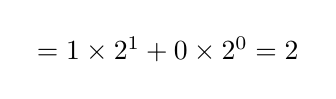
\begin{tikzpicture}
											\digits[thick](0.75:2:10:2)
											\node[] at (3.5,0.35) {$=1\times2^{1}+0\times2^{0}=2$};
										\end{tikzpicture}~\\
										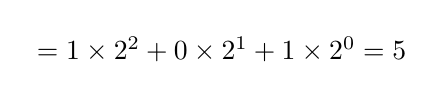
\begin{tikzpicture}
											\digits[thick](0.75:2:101:3)
											\node[] at (5.5,0.35) {$=1\times2^{2}+0\times2^{1}+1\times2^{0}=5$};
										\end{tikzpicture}~\\
										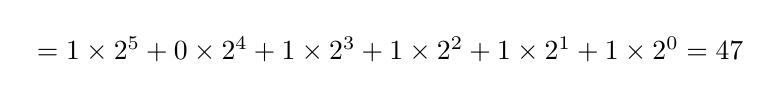
\begin{tikzpicture}
											\digits[thick](0.75:2:101111:6)
											\node[] at (10,0.35) {$=1\times2^{5}+0\times2^{4}+1\times2^{3}+1\times2^{2}+1\times2^{1}+1\times2^{0}=47$};
										\end{tikzpicture}
									\end{answer}
								}\fi
							\item Convert the following base-10 numbers to base-2: 5, 16, 109.
								\if\withsol1{
										\begin{answer}
											\begin{pycode}
from scripts import convert, vspace
convert(5,2)
vspace(1)
convert(16,2)
vspace(1)
convert(109,2)
											\end{pycode}
										\end{answer}
									}\fi

								\item Convert the same numbers to base-3 and base-16.
									\if\withsol1{
											\begin{answer}
												\begin{pycode}
from scripts import convert, vspace
convert(5,3)
vspace(1)
convert(16,3)
vspace(1)
convert(109,3)
												\end{pycode}
											\end{answer}
										}\fi

									\item How many bits are needed to represent two hexadecimal digits? How many different numbers can be represented with two hexadecimal digits?
										\if\withsol1{
												\begin{answer}
													two hexadecimal digits can represent $16^{2}=256$ different values. Since $2^{8}=256$, 8 binary digits are needed to represent 2 hexadecimal digits.
												\end{answer}
											}\fi

										\item Convert the following 4-digit binary numbers to hexadecimal numbers: 0000, 0110, 1100, 1111.
											\if\withsol1{
													\begin{answer}
														$0000_{2}=0_{16}$\\
														$0110_{2}=6_{16}$\\
														$1100_{2}=\text{C}_{16}$\\
														$1111=\text{F}_{16}$\\
													\end{answer}
												}\fi

											\item Convert the following 2-digit hexadecimal numbers to binary numbers: 04, 1E, A7, FF.
												\if\withsol1{
														\begin{answer}
															Each single digit hexadecimal number has a 4-bit representation:\\~\\
															\begin{center}
																\begin{tabular}{l l|l l}
																	Hex & Bin & Hex & Bin\\
																	\hline
																	0 & 0000 & 8 & 1000\\
																	1 & 0001 & 9 & 1001\\
																	2 & 0010 & A & 1010\\
																	3 & 0011 & B & 1011\\
																	4 & 0100 & C & 1100\\
																	5 & 0101 & D & 1101\\
																	6 & 0110 & E & 1110\\
																	7 & 0111 & F & 1111\\
																	\hline
																\end{tabular}
															\end{center}~\\~\\
															Therefore, each $N$-digit hexadecimal number can be converted to a $4N$-bit number by simply converting each digit separately. Thus (notice that the leading zeros are discarded):
															\begin{align*}
																\text{04}_{16}&=0000\ 0100=100_{2}\\
																\text{1E}_{16}&=0001\ 1110=11110_{2}\\
																\text{A7}_{16}&=1010\ 0111=10100111_{2}\\
																\text{FF}_{16}&=1111\ 1111=11111111_{2}
															\end{align*}\\~\\
															A common notation for hexadecimal numbers in many programming languages is \textbf{0x} preceding the number. For example, the above numbers would be written as \textbf{0x04}, \textbf{0x1E}, \textbf{0xA7} and \textbf{0xFF}.
														\end{answer}
													}\fi
												\item YouTube uses Base64 to generate unique ID numbers for each video on their servers \if\withsol1{\footnote{Watch \url{www.youtube.com/watch?v=gocwRvLhDf8} for more information. Also note the video's ID and watch more of Tom Scott's videos!}}\fi. To represent Base64 all 10 digits are used (0-9) plus all lowercase English letters (a-z) plus all uppercase English letters (A-Z) plus two more signs: '-' (minus) and '\_' (underscore). Since YouTube uses 11 digits per video ID - how many unique IDs can this method yield?
													\if\withsol1{
															\begin{answer}
																Since each of the 11 digits can have any value out of 64 (important: the order doesn't matter and characters can repeat) - the total number of possible combinations is $64^{11}=73,786,976,294,838,206,464$.
															\end{answer}
														}\fi
												\end{enumerate}


